\subsection{Information-Theoretic Abstraction}
\label{sec:abstraction}


Before we present our concrete polynomial commitment scheme based on groups of unknown order, we present the underlying information theoretic protocol that abstracts the concrete cryptographic instantiations. 
The purpose of this abstraction is two-fold: first, it provides an intuitive stepping stone from which presenting and studying the concrete cryptographic protocol is easier; and second, it opens the door to alternative cryptographic instantiations that provide the same interface but based on alternative hardness assumptions. %Like the underlying information theoretic protocol in FRI~\cite{ICALP:BBHR18}, this protocol operates by recursively dividing the working polynomial into two parts and then combining the two parts with a random weight.

Let $[\![ * ]\!] : \mathbb{Z}_p[X] \rightarrow \mathbb{S}$ be a homomorphic commitment function that sends polynomials over a prime field to elements of some set $\mathbb{S}$. Moreover, let $\mathbb{S}$ be equipped with operations $* + * : \mathbb{S} \times \mathbb{S} \rightarrow \mathbb{S}$ and $ * \cdot * : \mathbb{Z}_p[X] \times \mathbb{S} \rightarrow \mathbb{S}$ that accommodate two homomorphisms for $[\![ * ]\!]$:
\begin{itemize}[nolistsep]
    \item a \emph{linear homomorphism}: $a \cdot [\![f(X)]\!] + b \cdot [\![g(X)]\!] = [\![af(X) + bg(X)]\!]$
    \item a \emph{monomial homomorphism}: $X^d \cdot [\![f(X)]\!] = [\![X^d f(X)]\!]$.
\end{itemize}
For now, assume both prover and verifier have oracle access to the function $[\![*]\!]$ and to the operations $ * \cdot *$ and $* + *$. (Later on, we will instantiate this commitment function using groups of unknown order and an encoding of polynomials as integers.)

The core idea of the evaluation protocol is to reduce the statement that is being proved from one about a polynomial $f(X)$ of degree $d$ and its evaluation $y = f(z)$, to one about a polynomial $f'(X)$ of degree $d'=\lfloor\frac{d}{2}\rfloor$ and its evaluation $y' = f'(z)$. For simplicity, assume that $d+1$ is a power of $2$.
The prover splits $f(X)$ into $f_L(X)$ and $f_R(X)$ such that $f(X) = f_L(X) + X^{d'+1} f_R(X)$ and such that both halves have degree at most $d'$. The prover obtains a random challenge $\alpha \in  \mathbb{Z}_p$ from the verifier and proceeds to prove that $f'(X)=\alpha \cdot f_L(X) + f_R(X)$ has degree $d'$ and that $f'(z) = y' = \alpha y_L + y_R$ with $y_L = f_L(z)$ and $y_R = f_R(z)$. 

The proof repeats this reduction by using $f'(X),z,y'$ and $d'$ as the input to the next recursion step. In the final step, $f(X) = f$ is a constant and the verifier checks that $f=y$.% $f \equiv y \bmod p$. Note that $|f| <  (\frac{p}{2})^{\log_2(d+1)+1}$ so a representation of $f$ requires at most $\lceil \log_2(d+1) \cdot \log_2(p)\rceil$ bits.

The commitment function binds the prover to one particular polynomial for every commitment held by the verifier. In particular, at the start of every recursion step, the verifier is in possession of a commitment $[\![f(X)]\!]$ to $f(X)$. The prover provides commitments $[\![f_L(X)]\!]$ and $[\![f_R(X)]\!]$, and the verifier checks their soundness homomorphically by testing $[\![f(X)]\!] = [\![f_L(X)]\!] + X^{d'+1} \! \cdot \! [\![f_R(X)]\!]$. From these commitments, the verifier can also compute the commitment to $f'(X)$ homomorphically, via $[\![f'(X)]\!] = \alpha \! \cdot \! [\![f_L(X)]\!] + [\![f_R(X)]\!]$. In the last step, the verifier checks that the constant polynomial $f$ matches the commitment by computing $[\![f]\!]$ outright. 

\begin{comment}
These operations give rise to the following informal, diagrammatic description of the \eval protocol.

\begin{figure}[!ht]
\begin{mdframed}[userdefinedwidth=\textwidth]
\newcommand{\dollar}{\$}
\begin{minipage}{\textwidth}
	\begin{flushleft}
	(Information-theoretic-)$\pro{Eval}([\![f(X)]\!], z, y, d; f(X)):$
		\begin{itemize}[nolistsep]
			\item \textbf{if} $d = 0$ \textbf{then:}
			\item[] \begin{tikzpicture}
			\node[] (prover) at (-5, 0) {\prover};
			\node[] (verifier) at (5, 0) {\verifier};
			\draw[->] (-4, -1) -- (4, -1) node[above, midway] {$f = f(X)$};
			\node[anchor=north west, xshift=-2.5cm, yshift=-1cm] (verifier checks) at (verifier.south west) {\begin{tabular}{l}
				check $f \in \mathbb{Z}_p$ and $f = y$ \\
				and $[\![f]\!] = [\![f(X)]\!]$
			\end{tabular}};
			\end{tikzpicture}
			\item \textbf{if} $d > 0$ \textbf{then:}
		 	\begin{tikzpicture}
			\node[] (prover) at (-5, 0) {\prover};
			\node[] (verifier) at (5, 0) {\verifier};
			\node[anchor=north west] (prover computes) at (prover.south west) {\begin{tabular}{l}
				split $f(X)$ into $f_L(X)$ and $f_R(X)$ \\
				s.t. $f(X) = f_L(X) + X^{d'+1}f_R(X)$ \\
				compute $y_L \gets f_L(z)$ and $y_R \gets f_R(z)$
			\end{tabular}};
			\draw[->] (-4, -2.7) -- (4, -2.7) node[above, midway] {$y_L, y_R, [\![f_L(X)]\!], [\![f_R(X)]\!]$};
			\node[anchor=north west, xshift=-2.5cm, yshift=-2.5cm] (verifier checks) at (verifier.south west) {\begin{tabular}{l}
			check $[\![f(X)]\!] =$ \\
			 $[\![f_L(X)]\!] + X^{d'+1}\cdot [\![f_R(X)]\!]$ \\
			check $y = y_L + z^{d'+1}y_R$ \\
			sample $\alpha \xleftarrow{\dollar} \mathbb{Z}_p$
			\end{tabular}};
			\draw[->] (4, -5.5) -- (-4, -5.5) node[above, midway] {$\alpha$};
			\node[anchor=north west, yshift=-0.5cm] (verifier updates) at (verifier checks.south west) {\begin{tabular}{l}
				compute $y' \gets \alpha y_L + y_R$ \\
				compute $[\![f'(X)]\!] \gets$ \\
				$\alpha \cdot [\![f_L(X)]\!] + [\![f_R(X)]\!]$
			\end{tabular}};
			\node[anchor=north west, yshift=-4cm] (prover updates) at (prover computes.south west) {compute $f'(X) \gets \alpha f_L(X) + f_R(X)$};
			\draw[<->] (4, -8) -- (-4, -8) node[above, midway] {run $\eval([\![f'(X)]\!], z, y', d'; f'(X))$};
			\end{tikzpicture}
		\end{itemize}
		\end{flushleft}
\end{minipage}
\end{mdframed}
\end{figure}
\end{comment}

\begin{comment}
These operations give rise to the following informal pseudocode description of the \eval protocol.
\begin{mdframed}
Information-theoretic $\eval$ protocol, informal. \\
Common knowledge: $[\![f(X)]\!], y, z, d$ \\
Secret knowledge for \prover: $f(X)$ of degree $d$ \\
Statement: $y = f(z) \bmod p$ and $\deg(f(X)) = d$
	\begin{itemize}[nolistsep]
	    \item \textbf{if} $d > 0$ \textbf{then:}
		\item \pcind[1] \prover splits $f(X)$ into polynomials $f_L(X)$ and $f_R(X)$ of degree $d'=\frac{d+1}{2}-1$ such that $f(X) = f_L(X) + X^{d'+1}f_R(X)$
		\item \pcind[1] \prover sends $[\![f_L(q)]\!]$ and $[\![f_R(q)]\!]$ as well as $y_L \gets f_L(z) \bmod p$ and $y_R \gets f_R(z) \bmod p$ to \verifier
		\item \pcind[1] \verifier checks that $[\![f_L(q)]\!]+q^{d'+1} [\![f_R(q)]\!] = [\![f(q)]\!]$ and $y_L+z^{d'+1} y_R =y$
		\item \pcind[1] \verifier sends a random challenge $\alpha$ from $[-\frac{p-1}{2} ; \frac{p-1}{2}]$ to \prover
		\item \pcind[1] \prover and \verifier recurse on $[\![f'(q)]\!]=\alpha [\![f_L(q)]\!]+[\![f_R(q)]\!]$ for the statement $f'(z) = \alpha y_L + y_R \bmod p$ and $\deg(f'(X)) = d'$
		\item \textbf{if} $d=0$ \textbf{then:}
		\item \pcind[1] $\prover$ sends the constant $f$ to $\verifier$
		\item \pcind[1] $\verifier$ checks that $f$ is a small constant, that $[\![*]\!]$ evaluated in $f$ equals $[\![f]\!]$, and that $y = f \bmod p$
	\end{itemize}
\end{mdframed}
\end{comment}

\subsection{Integer Polynomial Encoding}
\label{sec:encoding}
\if 0
We propose using integer commitments in a group of unknown order as a concrete instantiation of the homomorphic commitment scheme required for the abstract protocol presented in Section~\ref{sec:abstraction}. At the heart of our protocol is thus an encoding of integer polynomials with bounded coefficients as integers, which also has homomorphic properties. Any commitment scheme which is homomorphic over integer polynomials is automatically homomorphic over $\ZZ_p[X]$ polynomials as well (by reducing integer polynomials modulo $p$). Polynomials over $\ZZ_p[X]$ can be lifted to integer polynomials in a canonical way by choosing representatives in $[0,p)$. Therefore, from here on we will focus on building a homomorphic integer encoding of integer polynomials, and how to combine this with a homomorphic integer commitment scheme. 

\paragraph{Strawman encoding} In order to encode integer polynomials over an odd prime field $\mathbb{F}_p$, we first lift them to the ring of polynomials over the integers by choosing representatives in $[0,p)$. In the technical overview (Section~\ref{sec:overview}) we noted that a polynomial $f \in \ZZ[X]$ with positive coefficients bounded by $q$ can be encoded as the integer $f(q)$.   
The coefficients of $f$ can be recovered via the base $q$ decomposition of $f(q)$. %Let $\ZZ(b):=\{x \in \ZZ: \vert x \vert  \leq b\}$ denote the set of integers with absolute value less than or equal to $b$.
This encoding is an injective mapping from polynomials in $\ZZ[X]$ of degree at most $d$ with positive coefficients less than $q$ to the set $[0, q^{d+1})$. The encoding is also \emph{partially} homomorphic. 
If $f$ is encoded as $f(q)$ and $g$ is encoded as $g(q)$ where coefficients of both $g, f$ are less than $q/2$, then the base-$q$ decomposition of $f(q) + g(q)$ gives back the polynomial $f + g$. 
By choosing a sufficiently large $q \gg p$ it is possible to perform several levels of homomorphic operations on encodings.

\paragraph{What goes wrong?} Unfortunately, this simple encoding scheme does not quite work yet for the protocol outlined in Section~\ref{sec:overview}. The homomorphic consistency checks ensure that if $[\![f_L(X)]\!]$ is a homomorphic integer commitment to the encoding of $f_L \in \ZZ[X]$, $[\![f_R(X)]\!]$ is a homomorphic integer commitment to the encoding of $f_R \in \ZZ[X]$, and both $f_L, f_R$ are polynomials with $q/2$-bounded coefficients, then $[\![f(X)]\!]$ is an integer commitment to the encoding of $f_L + X^{d'}f_R$. (Moreover, if $f_L(z) = y_L \bmod p$ and $f_R(z) = y_R \bmod p$ then $f(z) = y_L + z^{d'} y_R \bmod p$). 

However, the validity of $[\![f_L(X)]\!]$ and $[\![f_R(X)]\!]$ are never checked directly. 
The verifier only sees the opening of the commitment at the bottom level of recursion. If the intermediate encodings use integer polynomials with coefficients larger than $q/2$ the homomorphism is not preserved. Furthermore, even if $[\![f(X)]\!]$ is a commitment to $f^*(q)$ with positive $q$-bounded coefficients, an adversarial prover could find an integer polynomial $g^*$ that does not have positive $q$-bounded coefficients such that $g^*(q) = f^*(q)$ and $g^* \not\equiv f^* \bmod p$ (\emph{i.e}, $g^*$ with coefficients greater than $q$ or negative coefficients). 
The prover could then commit to $g^*_L(q)$ and $g^*_R(q)$, and recurse on $\alpha g^*_L(q) + g^*_R(q)$ instead of $\alpha f^*_L(q) + f^*_R(q)$. This would be non-binding. (For example $f^*(X)= q-1$ and $g^*(X)=X-1$, or $f^*(X) = q +1$ and $g^*(X) = X + 1$). 

\paragraph{Inferring coefficient bounds} So what can the verifier infer from the opened commitment $[\![f']\!]$ at the bottom level of recursion? The opened commitment is an integer $f' = \alpha f_L + f_R$. From $f'$, the verifier can infer a bound on the absolute value of the coefficients of the integer polynomial $f(X) = f_L + X f_R$, given that $f_L$ and $f_R$ were already committed in the second to last round. The bound holds with overwhelming probability over the randomness of $\alpha \in [0,p)$. This is reasoned as follows: if $f'_0 \leftarrow \alpha_0 f_L + f_R$ and $f'_1 \leftarrow \alpha_1 f_L + f_R$ such that $\max(|f'_0|, |f'_1|) < q / (2p)$ for some distinct $\alpha_0 \neq \alpha_1$, then $|f_L| \leq |f'_1 - f'_0| < q / p$ and $|f_R| \leq |\alpha_0 f'_1 - \alpha_1 f'_0| < q/2$. If no such pair exists, \emph{i.e.} the bound only holds for a unique $\alpha$, then there is a negligibly small probability $1/p$ that $f'$ would have passed the bound check.


\paragraph{What about negative coefficients?} 
As shown above, the verifier can infer a bound on the absolute values of $f_L$ and $f_R$, but still cannot infer that $f_L$ and $f_R$ are both \emph{positive} integers. Moreover, if $f_R > 0$ and $f_L < 0$, then it is still possible that $f_L + q f_R > 0$, and thus that there is a distinct $g \neq f$ with $q$-bounded positive coefficients such that $g(q) = f(q)$. For example, say $f_R = q/2$ and $f_L = -1$ then $f_L + q f_R = q^2/2 - 1$, and $\alpha f_L + f_R  = q/2 - \alpha > 0$ for every $\alpha \in [0,p)$. Yet, also $q^2/2 - 1 = g(q)$ for $g(X) = (q/2 - 1)X + q-1$. 

\paragraph{Ensuring injectivity} How can we ensure the encoding scheme is injective over polynomials with either positive/negative coefficients bounded in absolute value? Fortunately, it is a fact that if $|f_L| < q/2$ and $|f_R| < q/2$ then at least one coefficient of $g$ must be larger than $q/2$. In other words, if the prover had committed instead to $f^*_L$ and $f^*_R$ such that $g(X) = f^*_L + Xf^*_R$ then the verifier could reject the opening of $\alpha \hat{f}^*_L + \hat{f}^*_R$ with overwhelming probability based on its size. 


More generally, for every integer $z$ in the range $B = (-\frac{q^{d+1}}{2}, \frac{q^{d+1}}{2})$ there is a unique degree (at most) $d$ integer polynomial $h(X)$ with coefficients whose absolute values are bounded by $q/2$ such that $h(q) = z$. \emph{We prove this elementary fact below and show how the coefficients of $h$ can be recovered efficiently from $z$ (Fact~\ref{EncodingBijective})}. If the prover is committed to $h(q)$ at level $i$ of the protocol, there is a unique pair of integers polynomial $h_L$ and $h_R$ with coefficients of absolute value bounded by $q/2$ such that $h_L(q) + q^{\frac{d+1}{2}} h_R(q) = h(q)$, and if the prover recurses on any other $h_L^*$ and $h_R^*$ with larger coefficients then the verifier's bound check at the bottom level of recursion will fail with overwhelming probability. 

\paragraph{Optimization with negative coefficients} As we have seen, an adversarial prover can commit to polynomials with positive or negative coefficients. As an optimization, we can actually allow the honest prover to encode polynomials using a mixture of negative and positive coefficients as well. A polynomial $f(X) \in \ZZ_p[X]$ is lifted to an integer polynomial by replacing each coefficient of $f$ with its unique integer representative from $(-p/2,p/2)$ of the same equivalence class modulo $p$. Also, $\alpha$ can be chosen from $(-p/2, p/2)$, leading to a tighter bound on coefficient growth. This leads us to the following encoding scheme. 
\fi

In contrast to the highly simplified technical overview presented earlier, we prefer a balanced choice of integer representatives of $\mathbb{Z}_p$. This choice benefits a more natural reasoning about the growth of coefficients in an extraction argument. We refer the reader to full version of this paper~\cite{DARK/Supersonic:fullversion} for a more elaborate motivation.

\paragraph{Encoding scheme} Let $\ZZ(b):=\{x \in \ZZ: \vert x \vert  \leq b\}$ denote the set of integers with absolute value less than or equal to $b$.  Define $\ZZ(b)[X] := \{f \in \ZZ[X]: ||f||_\infty \leq b\}$, the set of integer polynomials with coefficients from $\ZZ(b)$. (For a polynomial $g \in \ZZ[X]$ the norm $||g||_\infty$ is the maximum over the absolute values of all individual coefficients of $g$).
\begin{itemize} 

\item \textbf{Encoding.}
For any integer $q$, the function $\mathsf{Enc} : \mathbb{Z}(b)[X] \rightarrow \mathbb{Z}$ maps $h(X) \mapsto h(q)$. A polynomial $f(X) \in \ZZ_p[X]$ is first mapped to $\ZZ(p/2)[X]$ by replacing each coefficient of $f$ with its unique integer representative from $(-p/2,p/2)$ of the same equivalence class modulo $p$.  %This means the map can be used as encoding of polynomials in the domain $\ZZ(b)[X]$ with $b<q/2$.

\item \textbf{Decoding.}
Decoding works as follows. Define the partial sum $S_k := \sum_{i=0}^k f_i q^i$ with $S_{-1} := 0$. Assuming $|f_i| < q/2$ for all $i$, observe that for any partial sum $S_k$ we have $|S_k|<\frac{q^{k+1}}{2}$. Therefore, when $S_k < 0$ then $S_k \bmod q^{k+1} > q^{k+1}/2$ and when $S_k \geq 0$ then $S_k \bmod q^{k+1} < q^{k+1}/2$. 
This leads to a decoding strategy for recovering $S_k$ from $y \in \mathbb{Z}$. The decode algorithm sets $S_k$ to $y \bmod q^{k+1}$ if this value is less than $q^{k+1}/2$ and to $q^{k+1}- (y \bmod q^{k+1})$ otherwise.
Two consecutive partial sums yield a coefficient of $f(X)$: $f_k = \frac{S_{k} - S_{k-1}}{q^{k}} \in \ZZ(b)$. These operations give rise to the following algorithm.\\
\end{itemize}

 \begin{minipage}{\textwidth}
\begin{mdframed}
\begin{flushleft}
	$\pro{Dec}(y \in \mathbb{Z}):$
	\begin{enumerate}[nolistsep]
	    \item \textbf{for each} $k$ \textbf{in} $[0, \, \lfloor \log_q(|y|)\rfloor]$ \textbf{do:}\\
		\item \pcind[1] $S_{k-1} \gets (y \bmod q^{k})$
		\item \pcind[1] \pcif{$S_{k-1} > q^{k}/2$} \textbf{then} $S_{k-1} \gets q^{k}-S_{k-1}$ \textbf{end if}
		\item \pcind[1] $S_k \gets (y \bmod q^{k+1})$
		\item \pcind[1] \pcif{$S_{k} > q^{k+1}/2$} \textbf{then} $S_{k} \gets q^{k+1}-S_{k}$ \textbf{end if}
		\item \pcind[1] $f_k \gets (S_{k} - S_{k-1}) / q^k$
		\item \pcreturn $f(X) = \sum_{k=0}^{\lfloor \log_q(|y|)\rfloor} f_k X^k$
	\end{enumerate} 
\end{flushleft}
\end{mdframed}
\end{minipage}

\begin{fact} \label{EncodingBijective}
Let $q$ be an odd integer. For any $z$ in the range $B = (-\frac{q^{d+1}}{2}, \frac{q^{d+1}}{2})$ there is a unique degree (at most) $d$ integer polynomial $h(X)$ in $\ZZ(\frac{q-1}{2})[X]$ such that $h(q) = z$. 
\end{fact}
\begin{proof}
Given any degree (at most) $d$ integer polynomial $f \in \ZZ(\frac{q-1}{2})$, by construction we see that $\pro{Dec}(\pro{Enc}(f)) = f$. Therefore, $\pro{Enc}$ is an injective map from degree (at most) $d$ polynomials in $\ZZ(\frac{q-1}{2})[X]$ to $B$. Furthermore, the cardinality of both the domain and range of this map is $q^{d+1}$. This shows that the map is surjective. In conclusion, the map is bijective. 
\end{proof}

\paragraph{Encoding of dyadic rational polynomials.}
There exists an algorithm to compute square roots of any element of a class group of an imaginary quadratic order, originally described by Gauß (see Bosma and Stevenhagen for a modern description~\cite{jtn/BosSte96}). As a result, in such class groups an adversary can also commit to \defn{dyadic rationals} $\mathbb{D}:=\{\frac{x}{2^k} : \ x \in \ZZ \wedge k \in \NN\}\subset \QQ$, in addition to integers. When using class groups we therefore need to modify the encoding scheme . 

The encoding map is identical, except lifted to the dyadic rationals: $\mathsf{Enc} : \mathbb{D}[X] \rightarrow \mathbb{D}, \, g(X) \mapsto g(q)$. The main difference with respect to the integer encoding scheme will be that decoding works for dyadic rationals where \emph{both the numerator and the denominator are bounded}. Let $N \in \NN$ be a bound on the absolute value of the numerator and $2^D\in \NN$ be a bound on the value of the denominator, and let $\mathbb{D}(N, D) :=\{\frac{x}{2^a} \in \mathbb{D} : \ |x|\leq N \wedge 2^a \leq D\}$ denote the set of such bounded dyadic rationals. The encoding scheme is uniquely decodable if $N \cdot 2^a < q/2$.
 
Note that denominator of $g(q)$ is bounded by $2^{\lfloor\log_2(D)\rfloor}$, $D$ rounded down to the next power of $2$. To decode such a dyadic rational, compute the integer $y \gets g(q) \cdot 2^{\lfloor\log_2(D)\rfloor}\in \ZZ$  and use the decoding algorithm described above to decode a polynomial $f(X)$ in $\ZZ(q/2)[X]$. From $f(X)$ one derives the polynomial  $g(X) \gets \frac{f(X)}{2^{\lfloor\log_2(D)\rfloor}} \in \mathbb{D}(\lceil q/(2D)\rceil, 2^{\lfloor\log_2(D)\rfloor})[X]$ through division. If the integer polynomial encoding is uniquely decodable, then so is the scheme for dyadic rational polynomials. If $q$ is a power of $2$, then an adversary can encode Laurent polynomials, \emph{i.e.}, polynomials where some terms have negative powers. In order to disallow negative powers, $q$ must be odd.

\subsection{Concrete Polynomial Commitment Scheme}
\label{subsec:concretepoly}
We now instantiate the abstract homomorphic commitment function $[\![ * ]\!]$. To this end we sample a group of unknown order $\mathbb{G}$, and sample a random element $\gr{g}$ from this group. 
Lift the field polynomial $f(X)\in \ZZ_p[X]$ to an integer polynomial with bounded coefficients, \emph{i.e.}, $\hat{f}(X)\in \ZZ(\frac{p-1}{2})[X]$ such that $\hat{f}(X)\bmod p=f(x)$.
We encode $\hat{f}(X)$ as an integer by evaluating it at a ``large enough'' integer $q$. Finally we use exponentiation in $\GG$ to commit to the integer. $[\![f(X)]\!]$, therefore, corresponds to $\gr{g}^{\hat{f}(q)}$. This commitment function inherits the homomorphic properties of the integer encoding for a limited number of additions and multiplications-by-constant. The monomial homomorphism for $X^d$ is achieved by raising the group element to the power $q^{d}$. To maintain consistency between the prover's witness polynomials and the verifier's commitments, the prover operates on polynomials with integer coefficients  $\hat{f}(X), \hat{g}(X)$, \emph{etc.}, without ever reducing them modulo $p$.

The $\setup, \pro{Commit}$ and $\open$ functionalities are presented formally below. Note that the scheme is parameterized by $p$ and $q$.
%; these values are determined by the context and independently of $\setup$.

%We now present our main technical contribution: a polynomial commitment scheme with an efficient evaluation protocol based on a group of unknown order $\GG$. For polynomials of degree $d=\poly$ the evaluation protocol uses $1+\lceil\log_2(d+1)\rceil$ rounds and $O(\log(d))$ communication and verifier work.

%Exponentiation in groups of unknown order is a succinct and homomorphic cryptographic commitments to an integer.
%Using the integer encoding of polynomials, or their encoding as dyadic rationals, above we can simply commit to a polynomial $f(X)$ with bounded coefficients by computing $\gr{g}^{f(q)} \in \GG$. Every polynomial in $\ZZ_p[X]$ naturally maps to an integer polynomial with coefficients in $B_{\frac{p-1}{2}}$. The commitment scheme, therefore, supports committing to polynomials in $\ZZ_p[X]$ for $p \leq q$. Interestingly, neither $p$ nor the degree $d$ need to be specified in the setup. 

%As long as $q$ and ``big enough'' they can be freely chosen.\alan{Todo: make this observation elsewhere.} %In class groups there is an efficient algorithm to compute square roots, and as a result, a prover can also commit to dyadic rationals. Since every dyadic rational corresponds to a unique element in $\ZZ_p$ we can simply extend the encoding to work for polynomials with bounded dyadic rational coefficients. The only difference is that we require $q$ to be odd such that the prover cannot commit to polynomials with negative powers. We will discuss the relationship between $p$, $d$ and $q$ in more detail later but first we describe the setup, commitment and opening algorithms:

\begin{itemize}
\item $\pro{Setup}(1^\secpar):$ Sample $ \GG \sample \ggen(\secpar)$
			and $ \gr{g} \sample \GG$. Return $\params = (\secpar,\GG,\gr{g}, q)$.
\item $\pro{Commit}(\params;f(X) \in \ZZ_p[X]):$ Compute $\gr{C} \gets \gr{g}^{\hat{f}(q)}$ and return $(\gr{C};\hat{f}(X))$.
\item $\pro{Open}(\params,\gr{C}, f(X), \hat{f}(X)):$ Check that $\hat{f}(X)\in \ZZ(q/2)[X]$ and $\gr{g}^{\hat{f}(q)} = \gr{C}$ and $f(X) = \hat{f}(X) \bmod p$. 
\end{itemize}

\begin{comment}
\begin{small}
\begin{mdframed}[userdefinedwidth=\textwidth]
\begin{minipage}{\textwidth}
	\begin{flushleft}
	$\pro{Setup}(1^\secpar):$
		\begin{enumerate}[nolistsep]
			\item $ \GG \sample \ggen(\secpar)$
			\item $ \gr{g} \sample \GG$
			%\item $q \gets 2^k$ such that $q > (d+1) \cdot 2\cdot p^{\log_2(d+1)+1} $
			%\item Pick a prime $p\in \NN$ such that $\lceil\log_2(p)\rceil=\lambda$.
			%\item Pick a sufficiently large and odd $q\in \NN$ (See discussion above)
			%\item $\pcreturn \params = (\secpar,\GG,\gr{g},p,q)$
			\item $\pcreturn \params = (\secpar,\GG,\gr{g})$
		\end{enumerate}
	$\pro{Commit}(\params;f(X) \in \ZZ(p)[X]):$ \pccomment{$f(X)\equiv \tilde{f}(X) \mod p$ for  $\tilde{f}(X)\in \ZZ_p[X]$}
		\begin{enumerate}[nolistsep]
			\item $\gr{C} \gets \gr{g}^{f(q)}$
			\item $\pcreturn (\gr{C};f(X))$
		\end{enumerate}
	$\pro{Open}(\params,\gr{C}, f(X)):$ \pccomment{$f(X) \in \ZZ(b)[X]\subset\mathbb{Z}[X]$ for $b<q/2$}
		\begin{enumerate}[nolistsep]
		    \item \prover sends $f(X)$ to \verifier.
		   % 				\item \verifier checks that $\tilde{f}(X) = f(X) \mod p$
		    \item \verifier checks that $f(X)\in \ZZ(b)[X]$ and $b<q/2$
			\item \verifier checks that $\gr{g}^{f(q)} = \gr{C}$ \pccomment{Can be outsourced using $\textsf{PoE}(\gr{g},\gr{C},f(q))$}
			\item \pcif all checks pass \textbf{then} \pcreturn $1$ \textbf{else} \pcreturn $0$
		\end{enumerate}
		\end{flushleft}
\end{minipage}
\end{mdframed}
\end{small}
\end{comment}
%Opening the commitment can be simply done by rerunning the commitment algorithm. Additionally a proof of exponentiation (PoE) can be used to increase verifier efficiency.
%The commitment inherits the homomorphic properties of the integer encoding. Assume that we are committing to representations of polynomials in $\ZZ_p[X]$, \emph{i.e.}, polynomials with coefficients bounded by $p$. Then the commitment scheme supports up to $\frac{q}{p}$ homomorphic additions. Equivalently, when raising a commitment to a weight $\alpha$, the size of the coefficients grows by at most a factor of $|\alpha|$. We use this property to build an efficient $\eval$ protocol. 

%The core idea of the $\eval$ protocol is to reduce the statement from one about a polynomial $f(X)$ of degree $d$ to one about a polynomial of degree $d'=\frac{d+1}{2}-1$. For simplicity assume that $d+1$ is a power of $2$.
%The prover splits $f(X)$ into $f_L(X)$ and $f_R(X)$ such that $f(X) = f_L(X)+X^{d'+1} f_R(X)$ and such that both polynomials have degree at most $d'$. Then he proves that $f'(X)=\alpha \cdot f_L(X) + f_R(X)$ has degree $d'$ for a random challenge $\alpha\in [-\frac{p-1}{2},\frac{p-1}{2}]$. 

%If the prover wants to show, in addition to the previous, that $f(z)=y\bmod p$, then he can simply provide $y_L=f_L(z)\bmod p$ and $y_R=f_R(z)\bmod p$ and show that $y_L + z^{d'+1} \cdot y_R \bmod p=y$. Note that the verifier can compute $y' = f'(z) = \alpha \cdot y_L + y_R \bmod p$ from $y_L$ and $y_R$.

%The proof recursively repeats this reduction by using $f'(X),z,y'$ and $d'$ as the input. In the final step, the prover simply sends the constant polynomial $f$ and the verifier can check that $f \equiv y \bmod p$. Note that $|f|< (\frac{p}{2})^{\log_2(d+1)+1}$ so an integer encoding of $f_0$ requires at most $\lceil \log_2(d+1) \cdot \log_2(p)\rceil$ bits. 
\paragraph{Evaluation protocol}
Using the cryptographic compilation of the information theoretic protocol we get an $\eval$ protocol with logarithmic communication. In every round, however, the verifier needs to check consistency between $[\![f_L(X)]\!],[\![f_R(X)]\!]$ and $[\![f(X)]\!]$. This is done by checking that $\gr{C}_L \cdot \gr{C}_R^{q^{d'+1}}=\gr{C}$. This naive check is highly inefficient as the exponent $q^{d'+1}$ has $O(d)$ bits.
%For the concrete evaluation protocol, one starts with the situation in which the verifier possesses a commitment to $f(X)$ in the form of $\gr{C} = \gr{g}^{f(q)}$. The prover commits to $f_L(X)$ and $f_R(X)$ by sending $\gr{C}_L$ and $\gr{C}_R$. The verifier checks that $\gr{C} = \gr{C}_L \cdot \gr{C}_R^{q^{d'+1}}$ and proceeds in the next step with the commitment $\gr{C}' = \gr{C}_L^\alpha \cdot \gr{C}_R$ to $f'(X)$. This instantiation produces an $\eval$ protocol with logarithmic communication. However, naïvely checking that $f(X) = f_L(X) + X^{d'+1} f_R(X)$ based on the commitments $\gr{C}, \gr{C}_L$ and $\gr{C}_R$ is inefficient because the bit-size of the exponent $q^{d'+1}$ is huge.
To resolve this inefficiency, we utilize a proof of exponentiation (\textsf{PoE})~\cite{ITCS:Pietrzak18,EC:Wesolowski19} to outsource the computation to the prover.
The \textsf{PoE} protocol is an argument that a large exponentiation in a group of unknown order was performed correctly. Wesolowski's \textsf{PoE}~\cite{EC:Wesolowski19} is public coin, has constant communication and verification time, and is thus particularly well-suited here.

We now specify subtleties that were previously glossed over. 
First, we handle the case where $d+1$ is not a power of 2.  Whenever $d+1$ is odd in the recursion, the polynomial is shifted by one degree --- specifically, $f'(X) = X f(X)$ and the protocol proceeds to prove that $f'(X)$ has degree bounded by $d' = d+1$ and evaluates to $y' = zy$ at $z$. The verifier obtains the matching commitment $\gr{C}'\gets\gr{C}^q$.

Second, the coefficients of $f(X)$ grow by a factor of $\frac{p+1}{2}$ in every recursion step, but eventually the transmitted constant $f$ has to be tested against some bound because if it is \emph{too large} it should be rejected. However, the function interface provides no option to specify the allowable size of coefficients. We therefore define and use a subroutine $\pro{EvalBounded}$, which takes an additional argument $b$ and which proves, in addition to what $\pro{Eval}$ proves, that all coefficients $f_i$ of $f(X)$ satisfy $|f_i| \leq b$. Importantly, $b$ grows by a factor for $\frac{p+1}{2}$ in every recursion step. This subroutine is also useful if commitments were homomorphically combined prior to the execution of $\pro{EvalBounded}$. The growth of these coefficients determines a lower bound on $q$: $q$ should be \emph{significantly} larger than $b$. Exactly which factor constitutes ``significantly'' is determined by the knowledge-soundness proof.

In the final round we check that the constant $f$ satisfies $|f|\leq b$ and the protocol's correctness is guaranteed if $b = \frac{p-1}{2}(\frac{p+1}{2})^{\lceil\log_2(d+1)\rceil}$. However, $q$ needs to be even larger than this value in order for extraction to work (and hence, for the proof of witness-extended emulation to go through). In RSA groups, where computing square roots is hard, we need $q>p^{2\log(d+1)+1}$; whereas in class groups where computing square roots is easy, we need $p^{3\log(d+1)+1}$. When this condition is satisfied, we can prove that the original committed polynomial has coefficients smaller than $\frac{q}{2}$. To avoid presenting two algorithms whose only difference is the one constant, we capture this constant explicitly in the variable $\boldsymbol{\varsigma}_{p,d}$ and set its value depending on the context:
\[
    \boldsymbol{\varsigma}_{p, d} = \left\{
        \begin{array}{ll}
            p^{\,\log_2(d+1)} & \quad \textnormal{(in RSA groups)} \\
            p^{\,2\log_2(d+1)} & \quad \textnormal{(in class groups)}
        \end{array}
    \right. \enspace .
\]

 We now present the full, formal $\eval$ protocol below.
%\begin{small}
\begin{figure}[!ht]
\begin{mdframed}
\begin{minipage}{\textwidth}
			$\pro{Eval}(\crs, \gr{C}\in \GG, z\in \ZZ_p, y\in \ZZ_p, d \in \NN; \tilde{f}(X)\in \ZZ_p[X]) :$ \pccomment{$\tilde{f}(X) = \sum_{i=0}^d \tilde{f}_i X^i$}
			\begin{enumerate}[nolistsep]
			\item \prover computes $f_i \in [-\frac{p-1}{2},\frac{p-1}{2}]$ such that $f_i\equiv \tilde{f}_i\bmod p$ for all $i\in[0,d]$.
			\item \prover computes $f(X)\gets \sum_{i=0}^d f_i \cdot X^{i}\in \ZZ(\frac{p-1}{2})[X]\subset \ZZ[X]$
			\item \prover and \verifier run $\pro{EvalBounded}(\params,\gr{C},z,y,d,\frac{p-1}{2};f(X))$
		    \end{enumerate}
		    		\vspace{1em}
		$\pro{EvalBounded}(\crs,\gr{C}\in \GG,z\in \ZZ_p,y\in \ZZ_p,d\in \NN,b\in \ZZ;f(X)\in \ZZ(b)[X])$		
	    \begin{enumerate}[nolistsep]
        \item \pcif $d=0$:
        \item \label{line:basestart}\pcind[1] \prover sends $f(X)\in \ZZ$ to the verifier. \pccomment{$f=f(X)$ is a constant}

        \item \pcind[1] \verifier checks that $b\cdot \boldsymbol{\varsigma}_{p,d} < q$\pccomment{$\boldsymbol{\varsigma}_{p,d}=O(p^{2\log(d)})$ (see Theorem~\ref{thm:polycommitsecurity} and \ref{thm:dyadicpolysecurity})}
        %q/(2^{\lceil \log_2(d+1) \rceil+1} p^{2 \lceil \log_2(d+1) \rceil+1})$
        \item \pcind[1] \verifier checks that $|f|\leq b$
          \item \pcind[1] \verifier checks that $f\equiv y \bmod p$
                \item \label{line:baseend}\pcind[1] \verifier checks that $\gr{g}^{f}=\gr{C}$
\item \pcind[1] \verifier outputs $1$ \pcif all checks pass, $0$ otherwise.
          \item \pcif{$d+1$ is odd}
         \item \pcind[1]  $d'\gets d+1, \gr{C}'\gets \gr{C}^q$, $y'\gets y\cdot z \bmod p$ and $f'(X)\gets X \cdot f(X)$.
         \item \pcind[1] \prover and \verifier run $\pro{EvalBounded}(\crs,\gr{C}',z,y',d',b;f'(X))$

        \item \pcelse: \pccomment{$d \geq 1$ and $d+1$ is even}
       
        \item \pcind[1] \prover and \verifier compute $d' \gets \frac{d+1}{2} - 1$
        \item \pcind[1] \prover computes $f_L(X) \gets \sum\limits_{i=0}^{d'} f_i \cdot X^i$ and $f_R(X)\gets\sum\limits_{i=0}^{d'} f_{d'+1+i}\cdot X^{i}$
        \item \pcind[1] \prover computes $y_L\gets f_L(z) \bmod p$ and $y_R\gets f_R(z)\bmod p$
        \item \pcind[1] \prover computes $\gr{C}_L \gets \gr{g}^{f_L(q)}$ and $\gr{C}_R \gets \gr{g}^{f_R(q)}$
        \item \pcind[1] \prover sends $y_L,y_R, \gr{C}_L, \gr{C}_R$ to \verifier. \pccomment{See Section \ref{subsec:optimization} for an optimization}
        \item \pcind[1] \verifier checks that $y=y_L+z^{d'+1}\cdot y_R \bmod p$, outputs $0$ if check fails.
        \item \pcind[1] \label{line:PoE} \prover and \verifier run $\pro{PoE}(\gr{C}_R, \gr{C}/\gr{C}_L, q^{d'+1})$\pccomment{Showing that $\gr{C}_L\gr{C}_R^{(q^{d'+1})}=\gr{C}$}
        \item \pcind[1] \verifier samples $\alpha \sample [-\frac{p-1}{2},\frac{p-1}{2}]$ and sends it to \prover
        \item \pcind[1] \prover and \verifier compute $y'\gets\alpha  y_L +y_R \bmod p$, $\gr{C}' \gets \gr{C}_L^\alpha  \gr{C}_R$, $b'\gets b \frac{p+1}{2}$. 
        \item \pcind[1] \prover computes $f'(X) \gets \alpha \cdot f_L(X) + f_R(X) \in \ZZ[X]$ \pccomment{$\deg(f'(X))=d'$}
        \item \pcind[1] \prover and \verifier run $\pro{EvalBounded}(\params, \gr{C}', z, y', d',b' ; f'(X))$
               \end{enumerate}
      \end{minipage}
\end{mdframed}
\end{figure}
%\end{small}


\begin{comment}
\end{comment}

\subsection{Security Analysis} 
 \newcommand{\bindinglemma}{
 The polynomial commitment scheme is binding for polynomials in $\ZZ(b)[X]$ for $b<q/2$ if either the Adaptive Root Assumption or the Strong RSA Assumption hold.
	}
\begin{lemma}
\label{lem:binding}
	\bindinglemma
	\end{lemma}

\newcommand{\correctnesslemma}{
The polynomial commitment scheme is correct for polynomials in $\ZZ_p[X]$ of degree at most $d$ if $q> p^{\lceil \log_2(d+1)\rceil+1}$.
}
 
 \begin{lemma}
 	\label{lem:correctness}
\correctnesslemma
 \end{lemma}


The proofs of the previous lemmas are in the full version of this paper~\cite[\S A.1 -- \S A.2]{DARK/Supersonic:fullversion}.
Next is the main security theorem, which states that the evaluation protocol has witness-extended emulation. We start with a high-level intuitive overview where we also identify potential obstacles.

\paragraph{Proof idea.} %Consider the information theoretic version of the $\eval$ protocol, where the prover sends the integer polynomials $f_L(X)$ and $f_R(X)$ in each round but the verifier does not read them.
The goal is to construct an extractor by recursively computing $f(X)$ from $f'(X)$. In the final round the verifier receives $f$ such that $|f| \leq b$, and therefore the extractor possesses this constant polynomial as well. Working backwards from here, the extractor uses rewinding in every step to find $f_L(X)$ and $f_R(X)$ and thereby finds $f(X) = f_L(X) + X^{d'+1}f_R(X)$.
Specifically, in each round the extractor has $f'(X)=\alpha f_L(X)+ f_R(X)$. Suppose the extractor also possesses $f''(X)=\alpha' f_L(X)+ f_R(X)$. From $f'(X)$, $f''(X)$, $\alpha$ and $\alpha'$ it is easy to compute $f_L(X)$ and $f_R(X)$. The extractor then computes $f(X)=f_L(X)+X^{d'+1} f_R(X)$.
A careful analysis shows that if the coefficients of $f'(X)$ are bounded by $b$ then $f_L(X)$ and $f_R(X)$ must have coefficients bounded by $b \cdot p$ in absolute value. Using a similar analysis we can show that $f(z)\bmod p=y$ for the extracted polynomial $f(X)$.

This argument shows that there is an extractor algorithm $\mathcal{X}$ capable of extracting the witness $f(X)$ from a binary tree of accepting transcripts. Moreover, a tree-finding algorithm $\mathcal{T}$ can output such a tree by repeatedly rewinding the prover, running it with fresh verifier randomness each time, and recording the resulting transcripts. As a result, the Generalized Forking Lemma~\cite{EC:BCCGP16} applies and establishes that the protocol has witness-extended emulation.

The full proof takes into account the cryptographic compilation of the protocol using the integer encoding and the commitment scheme based on groups of unknown order. Additionally the full proof will need to support dyadic rationals because taking square roots is easy in class groups.





%We are now in a position to prove the main security statement.

\newcommand{\maintheorem}{
The polynomial commitment scheme for polynomials in $\ZZ_p[X]$ of degree at most $d=\poly$, instantiated using $q>p^{2\lceil \log_2(d+1)\rceil+1}$ and $\ggen$, has witness extended emulation (Definition \ref{def:wee}) if the Adaptive Root Assumption and the Strong RSA Assumption hold for $\ggen$.
}
\begin{theorem}~\label{thm:polycommitsecurity} 
	\maintheorem
\end{theorem}

%\textit{Remark:}
%The bound on $q$ for correctness (Lemma \ref{lem:correctness}) is $O((\frac{p}{2})^{\log(d)})$ while the bound for soundness is $O((\frac{p}{2})^{2 \log(d)})$. It is not clear whether this gap can be closed. While the soundness analysis is tight for the worst case assumption on challenges it is possible that a probabilistic analysis could give a tighter result.

\newcommand{\dyadicmaintheorem}{
Let $\ggen$ generate groups $\GG$ of unknown order such that the order of $\GG$ is odd, and such there exists a PPT algorithm for taking square roots in $\GG$. The polynomial commitment scheme for polynomials in $\ZZ_p[X]$ of degree at most $d=\poly$, instantiated using $q>p^{3\lceil \log_2(d+1)\rceil +1}$ and $\ggen$, has witness extended emulation (Definition \ref{def:wee}) if the Adaptive Root Assumption and the  $2$-Strong RSA Assumption hold for $\ggen$.
}
\begin{theorem}
\label{thm:dyadicpolysecurity}	
\dyadicmaintheorem
\end{theorem}
The proof of Theorem~\ref{thm:dyadicpolysecurity} is nearly identical to the proof of Theorem~\ref{thm:polycommitsecurity} but the extracted polynomials are polynomials over the dyadic rationals and not over the integers. This requires the bound on $q$ to be larger by a factor of $p^{\log(d+1)}$. Both proofs are presented in the full version of this paper~\cite[\S A.3 -- \S A.4]{DARK/Supersonic:fullversion}.

\subsection{Optimizations, Extensions, and Comparison}
Out of space constraints, the present version of this paper omits a number of interesting but non-essential sections.
The full version of this paper~\cite{DARK/Supersonic:fullversion} presents a range of optimizations for greater prover and verifier efficiency and smaller proof size, as well as protocol extensions to achieve special properties. These properties include batched evaluation, multi-point evaluation, multi-variate polynomial evaluation, and zero-knowledge polynomial evaluation with hiding commitments. Their exact performance metrics are computed and presented in a table. Furthermore, the full version includes a comparison to three alternative strategies (and specific instances of these strategies) for generating polynomial commitment schemes, namely based on bilinear maps, based on discrete logarithms, and based on Merkle trees of Reed-Solomon codewords.
%\subsection{Optimizations}
%\label{subsec:optimization}
%We present several ideas for optimizing the performance of the $\pro{Eval}$ protocol.

\paragraph{Precomputation.} The prover has to compute powers of $\gr{g}$ as large as $q^d$. While this can be done in linear time, this expense can be shifted to a preprocessing phase in which all elements $\gr{g}^{q^i}, i \in \{1, \ldots, d_{\it max}\}$ are computed. Since for coefficient $|f_i|\leq -\frac{p-1}{2}$ this allows the computation of $\gr{g}^{f(q)}$ in $O(\lambda d)$ group operations as opposed to $O(\lambda d \log(d))$.
In addition to reducing the prover's workload, this optimization enables parallelizing it. The computation of the $\textsf{PoE}$ proofs can simiarly be parallelized. The prover can express each $Q$ as a power of $\gr{g}$ which enables pre-computation of powers of $\gr{g}$ and parallelism as described by Boneh~\emph{et al.}~\cite{C:BonBunFis19}.
%The elements $\gr{g}^{q^i}$ can themselves be accompanied by non-interactive $\mathsf{PoE}$s to establish their correct computation.

The pre-computation also enables the use of multi-scalar multiplication techniques~\cite{pippenger1980evaluation}. Boneh~\emph{et al.}~\cite{C:BonBunFis19} and Wesolowski~\cite{EC:Wesolowski19} showed how to use these techniques to reduce the complexity of the $\textsf{PoE}$ prover. The largest $\textsf{PoE}$ exponent $q^{\frac{d+1}{2}}$ has $O(\lambda d \log(d))$ bits. Multi-scalar multiplication can therefore reduce the prover work to $O(\lambda d)$ instead of $O(\lambda d \log(d))$.

%\paragraph{Early termination.} The protocol specifies the recursion ends when $d=0$, but the communication cost might be reduced if it terminates earlier. This reduction holds when the size of the fewer group elements $\gr{C}_L$ and $\gr{C}_R$ outweigh the size of the larger polynomial $f(X)$ instead of the constant $f$.

%\paragraph{Fiat-Shamir.} All the challenges of the verifier are public coin and as a result the protocol can be made non-interactive in the random oracle model with the Fiat-Shamir heuristic~\cite{C:FiaSha86}. This technique replaces each message of the verifier with the hash of all previous protocol messages, lifted to the appropriate domain. For the \textsf{PoE}s, it is beneficial to reuse the same $\ell$ across all \textsf{PoE}s and to compute this prime as the hash of the entire transcript after (dropping the $\ell$s and) replacing every instance of $\gr{Q}$ by its matching $\gr{C}_R^{q^{d'+1}}$ counterpart. This optimization requires that $\ell$ be transmitted as part of the proof so that the verifier can infer the $\gr{C}_R^{q^{d'+1}}$ and $\gr{C}_L$, and only after this inference can the verifier check that $\ell$ was computed correctly. The concrete benefit of this optimization is the reduced work for the verifier: previously he had to perform $\lceil\log(d+1)\rceil$ exponentiations of $q \bmod \ell$ to the power $d'+1$, whereas now he can do this task once and record the intermediate results.

\paragraph{Two group elements per round.} In each round the verifier has a value $\gr{C}$ and receives $\gr{C}_L$ and $\gr{C}_R$ such that $\gr{C}_L+q^{d'+1}\cdot \gr{C}_R=\gr{C}$. This is redundant. It suffices that the verifier sends $\gr{C}_R$. The verifier could now compute $\gr{C}_L\gets \gr{C} -q^{d'+1} \gr{C}_R$, but this is expensive as it involves an scalar multiplication by $q^d$. Instead, the verifier infers $q^{d'+1}\cdot \gr{C}_R$ from the \textsf{PoE}: the prover's message is $\gr{Q}$ and the verifier can directly compute $q^{d'+1}\cdot \gr{C}_R\gets \ell \cdot \gr{Q}+r\cdot \gr{C}_R$ for a challenge $\ell$ and $r\gets q^{d'+1} \bmod \ell$. From this the verifier infers $\gr{C}_L \gets \gr{C}-q^{d'+1} \cdot \gr{C}_R$. The security of $\textsf{PoE}$ does not require that $q^{d'+1}\cdot \gr{C}_R$ be sent before the challenge $\ell$ as it is uniquely defined by $\gr{C}_R$ and $q^{d'+1}$.
The same optimization can be applied to the non-interactive variant of the protocol. 

Similarly the verifier can infer $y_L$ as $y_L\gets y-z^{d'+1} y_R$. This reduces the communication to two group elements per round and 1 field element. Additionally the prover sends $f$ which has roughly the size of $\log(d+1)$ field elements, which increases the total communication to roughly $2\log(d)$ elements in $\GG$ and $2\log(d)$ elements in $\ZZ_p$. 

%When the $\mathsf{PoE}$s are made non-interactive, the prover can get away with producing only two group elements instead of three. With a naïve application of the Fiat-Shamir heuristic, the $\mathsf{PoE}$ proof consists of $(\gr{C}_R, \gr{C}_R^\star, \gr{Q})$ where $\gr{Q}$ is determined by $\ell$, which in turn is determined by hashing all previous protocol messages: $\ell \gets \mathsf{H}(\cdot \Vert \gr{C}_R \Vert \gr{C}_R^\star)$. The optimization sends $(\gr{C}_R, \gr{Q}, \ell)$ instead. The verifier can infer $\gr{C}_R^\star = \gr{C}_R^{(q^{d'+1} \bmod \ell)}$ and then test $\mathsf{H}(\cdots \Vert \gr{C}_R \Vert \gr{C}_R^\star) \stackrel{?}{=} \ell$. This optimization is particularly compatible with the previous batching of $\mathsf{PoE}$s optimization, because while there is a unique $\gr{Q}$ for each round, there need only be one $\ell$ for the entire $\eval$ protocol.

\paragraph{Evaluation at multiple points}
The protocol and the security proof extend naturally to the evaluation in a vector of points $\boldsymbol{z}$ resulting in a vector of values $\boldsymbol{y}$, where both are members of $\mathbb{Z}_p^k$. The prover still sends $\gr{C}_L\in \GG$ and $\gr{C}_R\in \GG$ in each round and additionally $\boldsymbol{y}_L,\boldsymbol{y}_R \in \ZZ^k_p$. In the final round the prover only sends a single integer $f$ such that $\gr{g}^{f}=\gr{C}$ and $f \bmod p=y$.

This is significantly more efficient than independent executions of the protocol as the encoding of group elements is usually much larger than the encoding of elements in $\ZZ_p$. Using the optimization above, the marginal cost with respect to $k$ of the protocol is a single element in $\ZZ_p$. If $\lambda=\lceil\log_2(p)\rceil$ is $120$, then this means evaluating the polynomial at an additional point increases the proof size by only $15\log(d+1)$ bytes.

\paragraph{Joining $\mathsf{Eval}$s.} 
In many applications such as compiling polynomial IOPs to SNARKs (see Section~\ref{sec:polyiop}) multiple polynomial commitments need to be evaluated at the same point $z$. 
This can be done efficiently by taking a random linear combination of the polynomials and evaluating that combination at $z$. The prover simply sends the evaluations of the individual polynomials and then a single evaluation proof for the combined polynomials. The communication cost for evaluating $m$ polynomials at $1$ point is still linear in $m$ but only because the evaluation of each polynomial at the point is being sent. The size of the eval proof, however, is independent of $m$. 
Taking a random linear combination does increase the bound on $q$ slightly, as shown in Theorem~\ref{thm:joined} which is presented below.

\[
\mathcal{R_\textsf{JE}}(\params) = \left\lbrace
\langle (\gr{C}_1,\gr{C}_2, z, y_1,y_2,d), (f_1(X), f_2(X)) \rangle
: \\
\begin{array}{l} 
\gr{C}_1, \gr{C}_2 \in \GG \\
z, y_1, y_2 \in \mathbb{Z}_p \\
f_1(X), f_2(X) \in \ZZ(b) \\
(\gr{C}_1,z,y_1,d) \in \mathcal{R_\textsf{Eval}}(\params) \\
(\gr{C}_2,z,y_2,d) \in \mathcal{R_\textsf{Eval}}(\params)
\end{array}
\right\rbrace
\]





\begin{mdframed}
	$\pro{JoinedEval}(\crs, \gr{C}_1, \gr{C}_2, z, y_1, y_2, d; f_1(X),f_2(X)) :$ \pccomment{$f_1(X), f_2(X) \in \ZZ(\frac{p-1}{2})[X]$} \\
%	Statement: $f_1(z)=y_1\bmod p \wedge f_2(z)=y_2\bmod p \wedge \gr{g}^{f_1(q)}=\gr{C}_1$ and $\gr{g}^{f_2(q)}=\gr{C}_2$
Statement: $(\crs,\gr{C}_1,\gr{C}_2,z,y_1,y_2,b,d)\in \mathcal{R}_{\pro{JE}}$
			\begin{enumerate}[nolistsep]
			\item $b=||f_1,f_2||_\infty$
        \item \verifier samples $\alpha \sample [0,2^\lambda)$ and sends it to \prover
			\item \prover and \verifier compute $\gr{C}'\gets \alpha \cdot \gr{C}_1+\gr{C}_2$ and $y'\gets \alpha \cdot y_1 +y_2 \bmod p$
			\item \prover computes $f'(X)\gets \alpha f_1(X) +f_2(X)$
			\item \prover and \verifier run $\pro{EvalB}(\params,\gr{C}',z,y',d,b\cdot 2^{\lambda};f'(X))$
		    \end{enumerate}
\end{mdframed}

\newcommand{\theoremjoined}{
The protocol $\pro{JoinedEval}$ is an interactive argument for the relation $\mathcal{R}_{\pro{JE}}$ and has perfect completeness and witness extended emulation if the Strong RSA and Order Assumption hold for $\ggen$ and if $q>(p-1)(\frac{p^2-1}{2})^{\lceil \log_2(d+1)\rceil+1}$ (e.g., $q > p^{2\log_2(d+1)+3}$). }
\benedikt{Theorem needs to be updated. Protocol as well}
\begin{theorem}
\label{thm:joined}
\theoremjoined
\end{theorem}
\begin{proof}
	Security directly follows from \cref{thm:mvariate} as $C_1,C_2$ is a binding virtual commitment to the bivariate polynomial $f_1+ Y \cdot f_2$. That is, $C=C_1+q^d \cdot C_2$ can be computed from $C_1,C_2$ thus if $C$ is a binding commitment then so is $(C_1,C_2)$. Further \pro{JoinedEval} is identical to an invocation of \pro{MultiEval} on input $(\alpha,z)$
\end{proof}
The proof is presented in Appendix~\ref{appendix:joined}.

We can additionally combine this optimization with the previous optimization of evaluating a single polynomial at different points. This allows us to evaluate $m$ polynomials at $k$ points with very little overhead. 
The prover groups the polynomials by evaluation points and first takes linear combinations of the polynomials with the same evaluation point and computes $y_1$ to $y_k$ using the same linear combinations. Then it takes another combination of the joined polynomials. In each round of the $\eval$ protocol the prover sends $y_{L,1}$ through $y_{L,k}$, i.e. one field element per evaluation point and computes $y_{R,1}$ through $y_{R,k}$. In the final step the prover sends $f$ and the verifier can check whether the final $y$ values are all equal to $f\bmod p$.
 This enables an $\eval$ proof of $m$, degree $d$ polynomials at $k$ points using only $2\log_2(d+1)$ group elements and $(1+k)\log_2(d+1)$ field elements.\benedikt{Adapt}
 
\paragraph{Evaluating the polynomial over multiple fields}
The polynomial commitment scheme is highly flexible. For example it does not specify a prime field $\ZZ_p$ or a degree $d$ in the setup. It instead commits to an integer polynomial with bounded coefficients. That integer polynomial can be evaluated modulo arbitrary primes which are exponential in the security parameter $\lambda$ as the soundness error is proportional to its inverse.
Note that $q$ also needs large enough such that the scheme is secure for the given prime $p$ and degree $d$ (see Theorem \ref{thm:polycommitsecurity}). The second condition, however, can be relaxed. A careful analysis shows that the challenges $\alpha$ just need to be sampled from an exponential space, \emph{e.g.}, $[0,2^{\lambda})$. So as long as $q>p \cdot 2^{\lambda\cdot 2\lceil \log_2(d+1)\rceil}$ for RSA groups or  $q>p \cdot 2^{\lambda \cdot 3\lceil \log_2(d+1)\rceil}$ for class groups one can evaluate degree $d$ polynomial with coefficients bounded by $2^\lambda$ over any prime field.

Additionally, the proof elements $\gr{C}_L$, $\gr{C}_R \in \GG$ are independent of the field over which the polynomial is evaluated. This means that it is possible to evaluate a committed polynomial $f(X) \in \ZZ(b)$ over two separate fields $\ZZ_{p}$ and $\ZZ_{p'}$ in parallel using only $2\log(d+1)$ group elements. 

%This property can be used to efficiently evaluate the polynomial modulo a large integer $m$ by choosing multiple $\lambda$ bit primes $p_1,\dots p_k$ such that $\prod_{i=1}^k p_i\geq m$ and using the Chinese Remainder Theorem to simulate the evaluation modulo $m$.




%\subsection{Multivariate Commitment Scheme}
%\label{sec:multivariate}
%
We can extend our polynomial commitment scheme to multivariate polynomials. The idea is simply to use higher degrees of $q$ to encode the next indeterminate. The protocol is linear in the number of variables and logarithmic in the total degree of the polynomial. For simplicity we only present a protocol for $\mu$-variate polynomials where the degree in each variable is $d$. The protocol extends naturally to different degrees per variable.

\paragraph{Encoding}
Let $q_i=q^{(d+1)^i}$ then $\hat{f}(q_1,\dots,q_\mu)\in \ZZ$ is an encoding of the multivariate polynomial $f(X_1,\dots,X_\mu)$ with maximum degree $d$. We use $\dec_{Multi}(f(q),\mu,d)$ to denote the decoding of an $\mu$-variate polynomial with degree exactly $d$ in each variable. The decoding algorithm simply uses the univariate decoding algorithm described in Section \ref{sec:encoding} to decode a univariate polynomial $\hat{h}(X)$ of degree $(d+1)^{\mu}-1$.
Then it associates each monomial of the univariate polynomial with a degree vector $(d_1,\dots,d_\mu)$ of the multivariate polynomial. The coefficient of the $i$th monomial becomes the coefficient of the $(d1,\dots,d_\mu)$-monomial, where $(d_1,\dots,d_\mu)$ is the base-$(d+1)$ decomposition of $i$. 
\paragraph{Protocols}
 Using this encoding we can naturally derive the multivariate commitment scheme and $\eval$ protocol. The $\eval$ protocol computes the univariate polynomials $f(q_1,\dots,q_{\mu-1},X_\mu)$ and then uses the univariate eval protocol to reduce the claim from a claim about an $\mu$-variate polynomial to one about an $(\mu-1)$-variate one. At the final step the prover opens the now constant polynomial and the verifier can check the claim. For example, the protocol would reduce a bivariate (say $X$ and $Y$) cubic polynomial to a univariate one (in $Y$) in two rounds of interaction and then reduce the degree of $Y$ using another two rounds.
 
 \begin{mdframed}[userdefinedwidth=\textwidth]
\begin{minipage}{\textwidth}
	\begin{flushleft}
	$\pro{MultiSetup}(1^\secpar):$
		\begin{enumerate}[nolistsep]
			\item $ \GG \sample \ggen(\secpar)$
			\item $ \gr{g} \sample \GG$
			%\item $q \gets 2^k$ such that $q > (d+1) \cdot 2\cdot p^{\log_2(d+1)+1} $
			%\item Pick a prime $p\in \NN$ such that $\lceil\log_2(p)\rceil=\lambda$.
			%\item Pick a sufficiently large and odd $q\in \NN$ \pccomment{$q=O_\lambda(p^{\mu \cdot \log(d)})$}
			\item $\pcreturn \params = (\secpar,\GG,\gr{g})$
		\end{enumerate}
	$\pro{MultiCommit}(\params;f(X_1,\dots,X_\mu) \in \ZZ(\frac{p-1}{2})[X_1, \ldots, X_\mu]\subset \ZZ[X_1, \ldots, X_\mu]):$ 		\begin{enumerate}[nolistsep]
			\item $d\gets \deg(f)$\pccomment{For simplicity assume $f(X_1,\dots,X_n)$ has degree $d$ in each variable}
			\item $q_i\gets q^{(d+1)^{i-1}}$ for each $i\in [\mu]$
			\item $\gr{C} \gets \gr{g}^{f(q_1,\dots,q_\mu)}$
			\item $\pcreturn (\gr{C};f(X_1,\dots,X_\mu))$
		\end{enumerate}
			\end{flushleft}
\end{minipage}
\end{mdframed}
 
 \begin{mdframed}
\begin{minipage}{\textwidth}
			$\pro{MultiEval}(\params, \gr{C}\in \GG, \boldsymbol{z}\in \ZZ^\mu_p,y \in \ZZ_p, d,\mu,b \in \NN; f(X_1,\dots,X_\mu)\in \ZZ(b)[X_1, \ldots, X_\mu]) :$
			\begin{enumerate}[nolistsep]
			\item \pcif{$\mu=1$} 
			\item \pcind[1] \prover and \verifier run $\pro{EvalBounded}(\params,\gr{C},z_1,y,d,b,x;f(X_1))$ 
			\item \pcelse
			\item \pcind[1] Let $\hat{f}(X_\mu)\gets f(q_1,\dots,q_{\mu-1},X_\mu)$
			\item \pcind[1] Let $\crs_\mu \gets \{\lambda,\GG,\gr{g},p,q_\mu\}$
			\item \pcind[1] \prover and \verifier run the univariate $\pro{EvalBounded}(\params_\mu,\gr{C},z_\mu,y,d,q_\mu;\hat{f}(X))$
			\item \pcind[2] \textbf{except:} when $d=0$, $f$ is not sent; instead the protocol returns its input at this point, \emph{i.e.}, $(\gr{C}',y',b')$ along with the prover's witness $f'(X_1,\dots,X_{\mu-1})=\dec_{Multi}(f,\mu-1,d)$ (Lines~\ref{line:basestart}-\ref{line:baseend} of $\pro{EvalBounded}$). 
			\item \pcind[1]$\boldsymbol{z}'\gets (z_1,\dots,z_{\mu-1})\in \ZZ_p^{\mu-1}$
			\item \pcind[1]\prover and \verifier run $\pro{MultiEval}(\crs,C',\boldsymbol{z}',y',d,\mu-1,b';f')$
		    \end{enumerate}
      \end{minipage}
\end{mdframed}
We only proof security under the strong RSA assumption. The security proof, however, directly extends to groups where taking square roots is easy under the $2$-Strong-RSA Assumption. In that case $q>p^{3\mu \log_2(d+1)+1}$ suffices.
\begin{theorem}[Multivariate Eval]
	The polynomial commitment scheme for multi-variate polynomials consisting of protocols $(\pro{MultiSetup},\pro{MultiCommit},\pro{MultiEval})$ has perfect correctness and witness extended emulation if the Adaptive Root Assumption and the Strong RSA Assumption hold for $\ggen$ for $\mu$-variate polynomials of degree $d$ and if $d^\mu=\poly$ if $q> p^{2 \mu \log_2(d+1)+1}$.
\end{theorem}
\begin{proof}
	Perfect correctness follows from the correctness of the univariate commitment scheme and the fact that the coefficients of the witness polynomial in the honest execution are less than $\frac{p-1}{2}p^{\mu \lceil\log(d+1)\rceil}<q/2$.
	
	To show witness extended emulation we use the forking lemma (Lemma \ref{lemma:GFL}) and build a polynomial time extractor algorithm $\mathcal{X}_{\pro{MultiEval}}$ that given a binary tree of transcripts of depth $\mu \cdot\lceil\log(d+1)\rceil$, extracts a witness. Each node corresponds to a different challenge $\alpha$ as described in the forking lemma. The tree consists of at most $(d+1)^{\mu}=\poly$ transcripts. 
	Lemma~\ref{lem:poe} states that the probability that an adversary can create any accepting transcript for which the $\textsf{PoE}$ can't be replaced by a direct check is negligible under the Adaptive Root Assumption.
We can therefore invoke the lemma to replace all \textsf{PoE} executions with direct verification checks that $\gr{C}_L\gr{C}_R^{q^{d'+1}}=\gr{C}$. 
%The lemma focuses on the univariate \pro{Eval} protocol but works identically for the multivariate protocol. 

In constructing $\mathcal{X}_{\pro{MultiEval}}$ we use the extractor $\mathcal{X}_{\pro{Eval'}}$ described in the proof of Theorem~\ref{thm:polycommitsecurity}. $\mathcal{X}_{\pro{Eval'}}$ computes, given a tree of transcripts for $\pro{Eval'}$ a valid witness of $\pro{Eval'}$ or a fractional root of $\gr{g}$ or an element of known order in $\GG$. We construct $\mathcal{X}_{\pro{MultiEval}}$ recursively invoking $\mathcal{X}_{\pro{Eval'}}$ once per degree $\mu$. The probability that a polynomial time adversary and a polynomial time extractor $\mathcal{X}_{\pro{Eval'}}$ can produce a fractional root or an element of known order in $\GG$ is negligible under the strong-RSA and the the adaptive root assumptions. From hence on we will consider the case where neither of these events happen.

We use the superscript $(i)$ to denote the inputs to $\pro{MultiEval}$ where $\mu=i$. 
If $\mu=1$ then the extractor $\mathcal{X}_{\pro{Eval'}}$ directly extracts $f^{(1)}(X)\in \ZZ(b)$, a univariate degree $d$ polynomial with coefficients bounded by $b=\frac{p-1}{2}p^{2 \lceil\log_2(d+1)\rceil}$ and such that $f(z)=y \bmod p$. Note that $q/2>b$ so the extraction succeeds.

For $\mu>1$, let's assume that $f^{(\mu-1)}(X_1,\dots,X_{\mu-1})\in \ZZ(b)$ is an extracted $\mu-1$ variate polynomial with degree $d$ in each variable such that $f^{(\mu-1)}(z_1,\dots,z_{\mu-1}) \bmod p=y'$.
Let $f'\gets \enc_{Multi}(f^{(\mu-1)}(X_1,\dots,X_{\mu-1})\in \ZZ$ be the encoding of $f^{(\mu-1)}(X_1,\dots,X_n)$, such that $\gr{C}^{(\mu-1)}\gets \gr{g}^{f'}$. Note that $f'$ is equivalent to an encoding of a univariate degree $(d+1)^{\mu-1}$ polynomial with the same coefficients as the multivariate polynomial. Let $g^{(\mu-1)}(X)=\dec(f')\in \ZZ(b)[X]$ be that polynomial. 
Using $g^{(\mu-1)}(X)$ as the witness the extractor $\mathcal{X}_{\pro{Eval'}}$ extracts a univariate degree $(d+1)^{\mu}$ polynomial $g^{(\mu)}(X)$ with coefficients in $\ZZ(b \cdot p^{\lceil\log(d+1)}\rceil)$. 
Let $f''\gets g^{(\mu)}(q)$ be the encoding of $g^{(\mu)}$ such that $\gr{C}^{(\mu)}=\gr{g}^{f''}$. Note that using the multivariate decoding algorithm $f''$ also encodes a $\mu$-variate degree $d$ polynomial, i.e. $f^{(\mu)}(X_1,\dots,X_\mu)\gets \dec_{Multi}(f'',\mu,d)$. The $X^i$th coefficient of $g^{\mu}(X)$ is the coefficient for the base monomial defined by the base-$(d+1)$ decomposition of $i$, i.e. $\prod_{j=1}^\mu  X_j^{\lfloor i/(d+1)^{j-1}\rfloor \bmod d+1 }$ in $f(X_1,\dots,X_\mu)$. Note that the extraction additionally guarantees that the polynomial evaluation is correct, i.e. $f(z_1,\dots,z_\mu)\bmod p=y$.

The final extracted polynomial has coefficients in $\ZZ(\frac{p-1}{2}p^{2\mu \lceil\log_2(d+1)\rceil})$. Since $q>p^{2\mu\lceil\log_2(d+1)\rceil+1}$ both the univariate and the multivariate decoding succeed and the extractor extracts a valid $\mu$-variate degree $d$ witness polynomial.
\end{proof}


%\subsection{Hiding Commitments and Zero-Knowledge Evaluation}
%\label{section:zeroknowlege}
%Many applications, such as the construction of ZK-SNARKs, require a polynomial commitment scheme where an evaluation leaks no information about the committed polynomial beyond its value at the queried point. To provide this we show how to build a hiding polynomial commitment along with a zero-knowledge evaluation protocol.

We start by defining what it means for a polynomial commitment scheme to be \emph{hiding}:

\begin{definition}
A commitment scheme $\Gamma = (\pro{Setup}, \pro{Commit}, \pro{Open})$ is \defn{hiding} if for all probabilistic polynomial time adversaries $\adv = (\adv_0, \adv_1)$, the probability of distinguishing between commitments of different messages is negligible:
\[
	\left| 1 - 2 \cdot \mathrm{Pr}\left[
		\hat{b} = b \ \middle| \ 
		\begin{array}{l}
			\params \gets \pro{Setup}(1^\lambda) \\
			m_0, m_1, \st \gets \adv_0(\params) \\
			b \sample \{0,1\} \\
			(c; r) \gets \pro{Commit}(\params, m_b) \\
			\hat{b} \gets \adv_1(\st, c)
		\end{array}
	\right] \right| \leq \negl \enspace .
\]
\end{definition}
If the property holds for all algorithms then we say that the commitment is \emph{statistically} hiding.
\paragraph{Hiding Polynomial Commitment}
We make the polynomial commitment described in Section~\ref{sec:protocol} hiding by adding a degree $d+1$ term with a large random coefficient. Let $B\geq |\GG|$ be a publicly known upper bound on the order of $\GG$. We will choose the blinding coefficient between $0$ and $B\cdot 2^\lambda$. Formally, the hiding commitment algorithm is described as follows:
\begin{itemize}
	\item $\pro{CommitH}(f(X) \in \ZZ_p[X]) \rightarrow (\gr{C}; \hat{f}(X), d, r)$. Lift $f(X) \in \mathbb{Z}_p[X]$ to $\hat{f}(X) \in \mathbb{Z}(\frac{p-1}{2})[X]$ and select random integer $r \sample [0,B\cdot 2^\lambda)$. Compute $d \gets \deg(f(X))$ and $\gr{C} \gets (\hat{f}(q)+q^{d+1} \cdot r)\cdot \gr{g}$ and return commitment $\gr{C}$ with secret opening information $\hat{f}(X), d, r$.
\end{itemize}

Let $\gr{h} \leftarrow q^{d+1}\cdot \gr{g}$. 
To argue that $\gr{C}$ is hiding, it suffices to show that $\gr{C}$ is computationally indistinguishable from a random element of $\langle \gr{g}\rangle$, the cyclic group generated by $\gr{g}$. In a setting with trusted-setup, in which the trusted party has a trapdoor to compute the order of $\gr{g}$ (e.g. RSA groups), the trusted party can select $q$ such that $\gr{g}$ and $\gr{h}$ generate the same subgroup. In this case, $\gr{h}^r$ for $r \sample [0, B\cdot 2^\lambda)$ has statistical distance at most $2^{-\lambda}$ from uniform in $\langle \gr{g} \rangle$, so long as $B \geq |\langle \gr{g} \rangle|$. 

%The random coefficient $r$ ensures that $\gr{C}$ is nearly indistinguishable from a random group element. Assume that $\gr{g}$ and $\gr{g}^{q^{d+1}}$ generate the same group with order $n=|\langle \gr{g}\rangle|$. The element $\gr{A}\gets\gr{g}^c$ for $c\sample [0,n)$ is uniformly random from this subgroup. If $r \sample [0,B\cdot 2^\lambda)$ and $B\geq n$ then $\gr{B}\gets \gr{g}^r$ has statistical distance at most $2^{-\lambda}$ from uniform. Consequently $\gr{C}$ is statistically negligibly far from a random group element. 

Unfortunately, in a setting without a trusted setup, $\gr{h}$ might only generate a subgroup of $\langle \gr{g} \rangle$. The commitment then becomes computationally hiding under a \emph{Subgroup Indistinguishability Assumption}\footnote{Brakersi and Goldwasser define subgroup indistinguishability assumptions in a related but slightly different way.}~\cite{C:BraGol10}: our precise assumption is that no efficient adversary can distinguish a random element of $\langle \gr{h} \rangle$ from $\langle \gr{g} \rangle$ for any non-trivial $\gr{h} \in \langle \gr{g} \rangle$. %If an adversary can distinguish $\gr{C}$ from a random element with probability more than $2^{-\lambda}$ then he must be able to distinguish the subgroup generated by $\gr{g}^{q^{d+1}}$ from the subgroup generated by $\gr{g}$. 
For simplicity, Theorem~\ref{thm:hiding} assumes that $\gr{g}$ and $\gr{h}$ generate the same group. 

If the condition $\langle \gr{g} \rangle = {q^{d+1}} \cdot \langle \gr{g}\rangle$ cannot be guaranteed then the security proof must be modified to show that an adversary that can efficiently distinguish commitments with non-negligible probability must be able to distinguish between random elements sampled from $\langle \gr{g} \rangle$ and random elements sampled from $\langle q^{d+1}\cdot \gr{g} \rangle$. The informal proof sketch is as follows. 
Suppose there exists a non-uniform distinguisher $D_{f,g}$ that can distinguish freshly generated commitments to $f$ and $g$ with non-negligible probability, then the non-uniform adversary $\mathcal{A}_{f,g}$ may be constructed as follows: upon receipt of $\gr{g}'$ sampled either from $\langle \gr{g} \rangle$ or from $\langle  q^{d+1}\cdot \gr{g}\rangle$, it sends $f(q)\cdot \gr{g}+ \gr{g}'$ and $g(q)\cdot \gr{g}+ \gr{g}'$ to the distinguisher $D_{f,g}$. 
In the case that $\gr{g}'$ was sampled from $\langle  q^{d+1}\cdot \gr{g} \rangle$ this is a statistical simulation of a pair of commitments to $f$ and $g$ respectively, hence the distinguisher should succeed with non-negligible probability. In the case that $\gr{g}$ was sampled from $\langle \gr{g} \rangle$, the pair is actually statistically indistinguishable, and thus the distinguisher must fail. Thus, $\mathcal{A}_{f,g}$ is able to distinguish from which group $\gr{g}'$ was sampled with non-negligible probability, contradicting the subgroup indistinguishability assumption. 

\begin{theorem}\label{thm:hiding}
The commitment scheme $\Gamma = (\pro{Setup}, \pro{CommitH}, \pro{Open})$ is statistically hiding if $B \gg |\mathbb{G}|$ and if $\langle \gr{g} \rangle = \langle q^{d+1}\cdot \gr{g} \rangle$; and it is binding if the commitment described in Section~\ref{subsec:concretepoly} is binding.
\end{theorem}

\begin{proof}
The hiding commitment is a commitment to a degree $d+1$ polynomial. It therefore directly inherits the binding property from the non-hiding scheme.

To show hiding, we use the fact that the uniform distributions $[0,b]$ and $[a,a+b]$ have statistical distance $\frac{a}{b}$, \emph{i.e.}, the probability that any algorithm can distinguish the distributions from a single sample is less than $\frac{a}{b}$. Similarly $\gr{C}\gets ({f(q)+r\cdot q^{d+1}}) \cdot \gr{g}$ for $r\sample[0,B\cdot 2^{\lambda})$ has statistical distance at most $2^{-\lambda}$ from a uniform element generated by $\gr{g}$ if $B\geq |\langle \gr{g}\rangle|$. This means that two polynomial commitments can be distinguished by any algorithm with probability at most $2^{-\lambda+1}$.
\end{proof}


\paragraph{Zero-Knowledge Evaluation Protocol}

We now build a zero-knowledge evaluation protocol, which is an \eval protocol for a hiding polynomial commitment. The zero-knowledge protocol shows that the prover must know a degree $d$ polynomial $f(X)$ with bounded coefficients such that $f(z)\bmod p = y$ but does not leak any other information about $f$. Formally, we will show that the interactive $\pro{ZK-Eval}$ argument is honest verifier zero-knowledge according to Definition~\ref{def:hvzk} by constructing an efficient simulator $\mathcal{S}$ that can generate a distribution of transcripts that is indistinguishable from honestly generated transcripts.

The idea for the $\pro{ZK-Eval}$ protocol is a simple blinding of the polynomial borrowed from Zero-Knowledge Sumcheck~\cite{EPRINT:ChiForSpo17} and Bulletproofs~\cite{EC:BCCGP16,SP:BBBPWM18}. Let $f(X)$ be the committed polynomial, using the hiding commitment scheme. The prover wants to convince the verifier that $f(z)\bmod p=y$. To do this the prover commits to a degree $d$ polynomial $r(X)$ with random coefficients. The prover also reveals $y'\gets r(z)\bmod p$. The verifier then sends a random challenge $c$ and the prover and verifier can compute a commitment to $s(X)\gets r(X)+c\cdot f(X)$. The random polynomial $r(X)$ ensures that $s(X)$ is distributed statistically close to a random polynomial. The prover could just reveal $s(X)$ and the verifier can check that $s(z)\bmod p=y'+c \cdot y\bmod p$. Instead of sending $s(X)$ in the clear, the prover can additionally just send the commitment randomness to provide the verifier with a non-hiding commitment to $s(X)$. The prover and verifier can then use the standard $\eval$ protocol to efficiently evaluate $s$ at $z$.
 \noindent\begin{mdframed}[userdefinedwidth=\textwidth]
\begin{minipage}{\textwidth}
	\begin{flushleft}
	\pro{ZK-Eval}$(\params, \gr{C} \in \GG, z \in \ZZ_p, y \in \ZZ_p, d \in \NN; f(X) \in \ZZ(b)[X], r \in \ZZ):$\\
		%Statement: $\langle(\gr{C},z,y,d),(f(X) \in \ZZ(\frac{p-1}{2})[X],r)\rangle \in \mathcal{R}_\eval(\params)$\\
	%Input: $\params,\gr{C} \in \GG,z,y \in \ZZ_p, b\in \ZZ,d$, Witness: $f(X) \ZZ(b),\alpha \in \ZZ(2^\lambda)$\\
	\begin{enumerate}[nolistsep]
		    \item \prover samples a random degree $d$ $k(X) \sample \ZZ(p\cdot 2^{2 \lambda})[X]$ and $r_k \sample [0,B\cdot 2^\lambda)$ and computes $\gr{R} \gets (k(q) + r_k \cdot q^{d+1})+\gr{g}$ and $y_k \gets k(z) \bmod p$
		    \item \prover sends $\gr{R}$ and $y_k$ to $\verifier$
		    \item \verifier samples random $c\sample [0,2^\lambda)$ and sends it to $\prover$
		    \item \prover computes $s(X)\gets k(X) + c \cdot f(X)$, as well as $r_s \gets r_k + c\cdot r$.
		    \item \prover sends $r_s$ to \verifier
		    \item \prover and \verifier compute $\gr{C}_s\gets \gr{R} + c\cdot \gr{C} +(-q^{d+1}\cdot r_s)\cdot \gr{g}$ and $y_s\gets y_k+c \cdot y \bmod p$ \pccomment{$\gr{C}_s=s(q)\cdot \gr{g}$}
		    \item \prover and \verifier run $\pro{EvalB}(\crs,\gr{C}_s,z,y_s,d,\frac{p^2}{4}\cdot 2^{\lambda+1};s(X))$ \pccomment{$s(z)\bmod p=y_s$}		   		\end{enumerate}
	\end{flushleft}
\end{minipage}
\end{mdframed}

\benedikt{update/wrong}

\begin{theorem}
	Let $\CSZ,\EBL$ and $\CorrectnessBound$ be defined as in \cref{thm:darkisdarkss} . Let  $\log q \geq 4(\lambda + 1 + \CSZ[\mu+1]) + \EBL[\mu+1] + \mathsf{CB}_{p^2\cdot 2^{\lambda},\mu+1,\lambda} + 1$.
Under the adaptive root assumption for $\ggen$, the \textsf{JoinedEval} protocol has witness-extended-emulation (\Cref{def:wee}) for the relation $\mathcal{R_\textsf{JE}}$.

Let  $\eval$ have perfect completeness and witness extended emulation for $q> b\cdot \boldsymbol{\varsigma}_{p, d}$. Assuming that $\pro{commitH}$ is statistically hiding and both the order assumption and the strong RSA assumption hold for $\ggen$ the protocol $\pro{EvalZK}$ has perfect completeness, witness extended emulation and $\delta$-statistical honest-verifier zero-knowledge for $q>2^\lambda\cdot (p-1)(\frac{p^2-1}{2})^{\lceil \log_2(d+1)\rceil+1}<p^{2\log_2(d+1)+4}$ and $\delta \leq d \cdot 2^{-\lambda}$.
\end{theorem}

\begin{proof}
A simple application of Theorem~\ref{thm:algebraicIOPcompiler} and Lemma~\ref{lem:intrandomcombine} shows that the protocol maintains witness extended emulation. The extractor extracts $s(X)$ and $s'(X)$ from the $\eval$ protocol for challenges $c$ and $c'$. We can directly use Lemma~\ref{lem:intrandomcombine} to extract the witness $f(X)$ or a break of an assumption from these two transcripts. The bound on $q$ grows by a factor of less than $p^2$ (or $p^3$ under the $2$-Strong RSA assumption).   

To show zero-knowledge, we build the simulator $\mathcal{S}$ as follows. Start with a polynomial $s(X) \sample \mathbb{Z}(\frac{p^2-1}{4})[X]$ with uniform random coefficients, and a blinding factor $r_s \sample [0,B\cdot 2^{2\cdot\lambda+1})$. The simulator $\mathcal{S}$ then chooses a random challenge $c \sample [0,2^\lambda)$ and computes $\gr{R} = (s(q) + r_s \cdot q^{d+1})\gr{g} -c\cdot \gr{C}$. The simulator then performs the rest of the $\eval$ protocol honestly using $s(X)$ as the witness. 

The randomizer $r_s$ is distributed identically to the honest $r_s$. Given the hiding property of the commitment scheme, $\gr{R}$ is statistically indistinguishable from any other commitment. Finally the simulated and the honest $s(X)$ have statistical distance at most $2^{-\lambda}$ from a random polynomial. The coefficients of $c\cdot f(x)$ are in $\ZZ(\frac{p^2}{4})$. The coefficients of the blinding polynomial $s(X)$ are sampled from a range that is larger by a factor $2^{\lambda}$. So the distribution of coefficients of $s(X) = k(X) + c \cdot f(X)$ is at a statistical distance at most $2^{-\lambda}$ away from the uniform distribution over $\ZZ(\frac{p^2}{4})$. Since the distributions of simulated and real coefficients are both uniform but merely over different sets, the statistical distance between the simulated $s(X)$ and the real $s(X)$ is at most $d \cdot 2^{-\lambda}$. The evaluation with $\pro{EvalB}$ cannot leak more than $s(X)$ itself. The views of the simulated and real transcripts are, therefore, $\delta$-close with $\delta \leq d \cdot 2^{-\lambda}$. Consequently, the protocol has $\delta$-statistically honest verifier zero-knowledge.
\end{proof}


\if 0
\subsection{Performance}
The polynomial commitment scheme has logarithmic proof size and verifier time in the degree $d$ of the committed polynomial. 
It has highly batchable proofs and it is possible to evaluate $n$ degree $d$ polynomials at $k$ points using only $2\log_2(d+1)$ group elements and $(k+1)\log_2(d+1)$ field elements. Note that this means the proof size is independent of $n$ and linear in $k$ but with a small constant $(15 \log(d)$ bytes). 
We describe the performance of our scheme for different settings in Table~\ref{tab:performance}.

\begin{table}[!htp]
\begin{small}
\begin{tabular}{l|l||l|l|l}
	Operation & $|\crs|$  & Prover & Verifier & Communication\\
	\hline
    $\pro{Commit}(f(X))$ & 1 $\GG$ & $O(\lambda d\log(d))\GG$ & - & $1 \GG$\\
    $\pro{Commit}(f(X))$ & $d$ $\GG$ & $O(\frac{\lambda d}{\log(d)}) \GG$ & - & $1 \GG$\\
    $f(z)=y\in \ZZ_p$  & 1 $\GG$ & $O(\lambda  \log(d) d)\GG$ & $O(\lambda \log(d))\GG$ & $2 \log(d) \GG$ +$2 \log(d) \ZZ_p$ \\
      $f(z)=y\in \ZZ_p$  & $d$ $\GG$ & $O(\lambda d)\GG$ & $O(\lambda \log(d))\GG$ & $2 \log(d) \GG$ +$2 \log(d) \ZZ_p$ \\
%    \eval($f(\boldsymbol{z})=\boldsymbol{y}\in \ZZ^k_p$)  & 1 $\GG$ & $O(\lambda \log(d)d)\GG$ & $O(\lambda \log(d))\GG$ & $2 \log(d) \GG$ +$(k+1) \log(d) \ZZ_p$ \\
       $f(\boldsymbol{z})=\boldsymbol{y}\in \ZZ^k_p$  & $d$ $\GG$ & $O(\lambda d)\GG$ & $O(\lambda \log(d))\GG$ & $2 \log(d) \GG$ +$(k+1) \log(d) \ZZ_p$ \\
  %      \eval($f(z)=y, g(z)=y'\in \ZZ_p$)  & $1$ $\GG$ & $O(\lambda\log(d) d)\GG$ & $O(\lambda \log(d))\GG$ & $2 \log(d) \GG$ +$2 \log(d) \ZZ_p$ \\
                $f(z)=y, g(z)=y'\in \ZZ_p$  & $d$ $\GG$ & $O(\lambda d)\GG$ & $O(\lambda \log(d))\GG$ & $2 \log(d) \GG$ +$2 \log(d) \ZZ_p$ \\

\end{tabular}

\caption{$\GG$ denotes the size of a group element for communication and a single group operation for computation. $\ZZ_p$ denotes the size of a field element, \emph{i.e.}, $\lambda$ bits. $|\crs|$ is the size of the public parameters (which is greater than one $\GG$ when preprocessing is used), and $d$ the degree of the polynomial. Rows 3-6 are for $\eval$ proofs of different statements.}
\label{tab:performance}
\end{small}
\end{table}
\fi

\if 0
\subsection{Comparison to Other Polynomial Commitment Schemes}

\subsubsection{Based on Pairings}

The polynomial commitment by Kate~\emph{et al.}~\cite{AC:KatZavGol10} has evaluation proofs that consist of only a single element in a bilinear group and verifying an evaluation requires only a single pairing computation. However, this asymptotically optimal performance comes at the cost of a trusted setup procedure that outputs a structured reference string whose size is linear in the degree of the polynomial. Our DARK polynomial commitment scheme requires no trusted setup but pays for this reduced trust requirement with a proof size and verification work that scale logarithmically in the degree of the polynomial.

In the multivariate setting, our scheme is logarithmic in the total number of coefficients: $\mu\log(d)$ for a $\mu$-variate polynomial of degree $d$ in each variable. The multivariate extension of Kate~\emph{et al.}'s commitment scheme~\cite{SP:ZGKPP17} evaluation proofs consist of $\mu$ group elements.

\subsubsection{Based on Discrete Logarithms}

\textsf{Bulletproofs}~\cite{EC:BCCGP16,SP:BBBPWM18} is a proof system based on prime order groups in which the discrete logarithm is hard. As a core component it relies on an inner product argument which can be used as a polynomial commitment (see \cite{SP:WTSTW18}). The polynomial commitment has logarithmic evaluation proofa with great constants. Unfortunately, the verifier time is linear in the size of the polynomial, i.e. $(d+1)^\mu$ for a $\mu$- variate degree $d$ polynomial.
The more general version of the commitment~\cite{EC:BCCGP16} can also give evaluation proofs with square root verifier time and square root proof size.


\subsubsection{Based on Merkle Trees of Reed-Solomon Codewords} \label{subsection:fri}

The FRI protocol~\cite{ICALP:BBHR18} is an efficient interactive oracle proof (IOP) that a committed oracle is close to a Reed-Solomon codeword, meaning that the prover commits to large sequences of field elements and the verifier queries only a few specific elements rather than reading the entire sequence. The abstract functionality is cryptographically compiled with a Merkle tree, which results in constant-size commitments and element queries that are logarithmic in the length of the codeword, \emph{i.e.}, the size of the oracle. FRI has been used in multiple recent zero-knowledge proof systems such as  \textsf{STARK}~\cite{C:BBHR19}, \textsf{Aurora}~\cite{EC:BCRSVW19}, and \textsf{Fractal}~\cite{Fractal}.

Since this oracle is a Reed-Solomon codeword, it represents the evaluations of a low-degree polynomial $f$ on an evaluation set $S \subset \FF$. In order to be used as a polynomial commitment scheme, the protocol needs to permit querying the polynomial outside of the evaluation set. DEEP-FRI~\cite{DEEPFRI} shows that this is possible and a recent note by Vlasov and Panarin \cite{MatterLabs} makes the connection explicit by building a polynomial commitment scheme from FRI. 
This FRI-based polynomial commitment scheme has evaluation proofs of size and verifier time $O(\lambda \log^2(d))$ where $\lambda$ is the security parameter and $d = \deg(f)$. To date, no extension to multivariate polynomials exists for FRI. The commitment relies only on symmetric cryptography and is plausibly quantum resistant.

\subsubsection{Comparison}

In Table \ref{tab:polycommit} we give a comparison between different polynomial commitment schemes in the literature. In particular, we evaluate the size of the reference string ($|\params|$), the prover and verifier time, as well as the size of the evaluation proof ($|\pi|$). Column $2$ indicates whether the setup is transparent, \emph{i.e.}, whether the reference string is structured. The symbol $\GG_U$ denotes a group of unknown order, $\GG_{B}$ a group with a bilinear map (pairing), and $\GG_{P}$ a group with prime (and known) order. Furthermore, $\textsf{EXP}$ refers to exponentiation of a $\lambda$ bit number in these groups, and $\hash$ is either the size of a hash output, or the time it takes to compute a hash, depending on context. 

Note that even when precise factors are given, the numbers should be interpreted as estimates. For example we chose to not display smaller order terms.
Note also that the prover time for the group based schemes could be brought down by a log factor when using multi-exponentiation techniques.

\begin{table}[!htp]
\begin{small}
\begin{tabular}{l||l|l|l|l|l}
	Scheme & Transp. & $|\crs|$  & Prover & Verifier & $|\pi|$ \\
	\hline
	\hline
    DARK  \textit{(this work)} & yes & $O(1)$ & $O( d^\mu \mu \log(d) )\; \textsf{EXP}$ & $3\mu \log(d)~\textsf{EXP}$ & $2 \mu \log(d) \; \GG_{U}$ \\
    Based on Pairings & no & $d^\mu$ $\GG_{B}$ & $O(d^\mu)\; \textsf{EXP}$  & $\mu\; \textsf{Pairing} $ & $\mu \; \GG_{B}$\\
    \cite[$\sqrt{\cdot}$]{EC:BCCGP16} & yes & $\sqrt{d^\mu}\GG_{P}$ & $O(d^\mu)$ \textsf{EXP} & $O(\sqrt{d^\mu})\textsf{EXP}$ &$O(\sqrt{d^\mu}) \; \GG_P$\\
       \textsf{Bulletproofs} & yes &$2 d^\mu\GG_{P}$& $O(d^\mu)$ \textsf{EXP}& $O(d^\mu)\textsf{EXP}$ &$2 \mu \log(d) \; \GG_P$\\
       FRI  ($\mu = 1$) & yes & $O(1)$ & $O(\lambda  d)$ $\hash$ & $O(\lambda \log^2(d))$ $\hash$ & $O(\lambda \log^2(d)) \; \hash$
\end{tabular}

\caption{Comparison table between different polynomial commitment schemes for an $\mu$-variate polynomial of degree $d$.}

\label{tab:polycommit}
\end{small}
\end{table}
\begin{comment}
	Multiple recent concrete proof systems such as use probabilistic testing of Reed-Solomon codes as
Recent years have seen a flurry of developments related to probabilistic testing of Reed-Solomon code membership~\cite{SIAMCOMP:BS08,STOC:BCGT13,ECCC:BGR16,ICALP:BBHR18,DEEPFRI}. Of these developments, the FRI~\cite{ICALP:BBHR18} protocol and its improvement DEEP-FRI~\cite{DEEPFRI} have seen deployment in concrete proof systems such as \textsf{STARK}~\cite{C:BBHR19}, \textsf{Aurora}~\cite{EC:BCRSVW19}, and \textsf{Fractal}~\cite{Fractal}. While these general purpose zero-knowledge proof systems do not use FRI as a polynomial commitment scheme, FRI does admit an interpretation as a one, as explained in a recent eprint note~\cite{MatterLabs}. In addition to that, mechanics that make FRI work are somewhat similar to the mechanics underlying our DARK polynomial evaluation protocol.

FRI stands for \emph{\underline{F}ast \underline{R}eed-Solomon \underline{I}OPP}, where IOPP stands for \emph{\underline{I}nteractive \underline{O}racle \underline{P}roof of \underline{P}roximity}. In such an information theoretical proof system, the prover sends sequences of field elements to the verifier and the verifier, rather than reading every sequence in its entirety, reads a select few random field elements from each sequence before sending a challenge back. At the end of the protocol the verifier should accept if the first sequence belongs to a given code, and he should reject if it is far from the code, under some precise definition of distance. We do not care what happens if the sequence has a small but nonzero distance from the nearest codeword. In order to simulate the verifier's random access in a concrete setting, the protocol is typically cryptographically compiled by representing every sequence as a Merkle tree: the prover sends the Merkle root, the verifier selects a random index, and the prover provides the authentication path for the field element located at that index.

A Reed-Solomon code $\mathsf{RS}[\mathbb{F}, S, \rho]$ is the set sequences of length $N = |S|$ of evaluations of some polynomial $f(X) \in \mathbb{F}[X]$ of degree at most $d < \rho N$ on an evaluation set $S \subset \mathbb{F}$. The rate parameter $\rho \in (0; 1]$ is typically 1/8 or on that order of magnitude. Note that \emph{any} Reed-Solomon IOPP can be turned into a polynomial commitment scheme. If it is true that $f(z) = y$ for some $z,y \in \mathbb{F}$ known to the verifier, then $X-z$ divides $f(X)-y$ and the relation for $f'(X) = \frac{f(X)-y}{X-z}$ can be probabilistically tested by reading the codewords for $f$ and $f'$ in a random $s \in S$. Moreover, $f'$ has degree at most $d-1$, so the protocol can recurse to prove that the codeword of $f'$ belongs to a \emph{smaller} code.

While Reed-Solomon IOPPs naturally extend to polynomial evaluation proofs, and hence to polynomial commitment schemes, for many purposes this extension is overkill. It suffices instead to prove membership in the code, or in other words, to establish a bound on the degree of the polynomial $f(X)$. FRI establishes this bound as follows. Let $S$ be a multiplicative subgroup of even order of $\mathbb{F} \backslash \{0\}$. In every iteration, the working polynomial $f(X)$ is split into two polynomials of degree at most $d' = \frac{d+1}{2}-1$, namely $f_E(X)$ and $f_O(X)$, such that $f(X) = f_E(X^2) + Xf_O(X^2)$. The verifier chooses a random weight $\alpha \in \mathbb{F}$ and the prover responds with (a Merkle tree commitment to the codeword matching) the polynomial $f'(X) = f_E(X) + \alpha f_O(X)$. Observe that for any square\footnote{In binary fields, where non-squares do not exist, the polynomial $f(X)$ is split into two halves based on a different two-to-one map from $X \mapsto X^2$; as such, $y, s_0, s_1$ and $S$ must be chosen accordingly.} $y \in \mathbb{F}$ and distinct square roots $s_0, s_1$ of $y$, the points 
\begin{flalign*}
    (s_0, f(s_0)) &= (s_0, f_E(y) + s_0f_O(y)) \\
    (s_1, f(s_1)) &= (s_1, f_E(y) + s_1f_O(y)) \\
    (\alpha, f'(y)) &= (\alpha, f_E(y) + \alpha f_O(y))
\end{flalign*}
lie on a straight line. The verifier can probabilistically test this collinearity by sampling $s_0, s_1, y \in S$ such that $s_0^2 = s_1^2 = y$, and querying the codewords. If this consistency test passes, the protocol recurses to establish that $f'(X)$ has degree at most $d'$. In the final round, $f'$ is a constant and is sent to the verifier.

Compared to our DARK evaluation protocol, the recursion principle is similar: split the working polynomial into two halves and combine them with a random weight. However, the consistency check is starkly different and matches the cryptographic tools that enable the compact representation of arbitrarily large polynomials, \emph{i.e.}, Merkle trees of Reed-Solomon codewords versus integer commitments in a group of unknown order. As a result, FRI has $O((\log d)^2)$ proof size and verifier time, whereas for DARK these quantities are only $O(\log d)$. Neither scheme requires a trusted setup. To date, FRI has no support for multivariate polynomials whereas for DARK this support is native.
\end{comment}

%\subsection{Multivariate polynomial commitments}\label{sec:multivariate}
	
\fi


